\documentclass[10pt,a4paper]{article}
\usepackage[utf8]{inputenc}
\usepackage{amsmath}
\usepackage{amsfonts}
\usepackage{amssymb}
\usepackage{tikz}
\usetikzlibrary{datavisualization}
\usetikzlibrary{datavisualization.formats.functions}
\usepackage[left=25mm,right=25mm]{geometry}
\usepackage{pgfplots}

\begin{document}

\newenvironment{indentPar}[1]%
 {\begin{list}{}%
         {\setlength{\leftmargin}{#1}}%
         \item[]%
 }
 {\end{list}}

\begin{flushleft}
\begin{LARGE}EE 535 Lab 1: Introduction to Transmission, Reflection, and Absorbance of Wafers and Thin Films
\end{LARGE}
\\Jonathan Hess
\end{flushleft}


\section*{Abstract}
\begin{indentPar}{1cm}
The band gap of a semiconductor defines its properties. Band gap of semiconductors can be measured by the absorption and reflection of light.
\end{indentPar}


\section*{Introduction}
\begin{indentPar}{1cm}
Three wafers were loaded into a spectrometer to measure their optical properties. These measured properties allowed for the calculation of band gap and whether the band gap is direct or indirect. The band gap of of a material determines its conductivity or in the case of an LED or solar panel what frequency of light it will produce/absorb. Determining if the band gap is direct would inform if any energy is required from the lattice structure whereas indirect wouldn't require this extra energy.
\end{indentPar}



\section*{Experimental}
\begin{indentPar}{1cm}
In this lab we measured the band gap through measurements of reflection and absorption. These measurements were done with the Cary 5000. This spectrometer works by comparing two slides. This allows to remove influence of the glass on the wafer's absorbtion and transmition.
\end{indentPar}


\section*{Theory}
\begin{indentPar}{1cm}
\begin{indentPar}{1cm}
$Transmition = T$ - \% of light 
$\\Reflectance = R$ - \% of light
$ \\Absorbance coefficient = \alpha \\ $
$\\Reflection =$ Intensity of neglected light
$\\A= \dfrac{|I_a|}{|I|}$
 For direct Eg $\alpha =(hv-Eg)^{1/2}\\T = (1-R^2)e^{-\alpha t}\\ \alpha = (1/t)ln((1-R^2)/T)$
\\
\end{indentPar}

These equations equations were derived from and the provided CSV output files were used inside a python script.
\end{indentPar}
\section*{Results}
\begin{indentPar}{1cm}
After running the spectrometer there were data points for the three wafers. These datapoints included transmition, reflection, and absorption the following graphs.
\\

    \begin{tikzpicture}
      \begin{axis}[
          width=\linewidth, % Scale the plot to \linewidth
          grid=major, % Display a grid
          grid style={dashed,gray!30}, % Set the style
          xlabel=hv(Ev), % Set the labels
          ylabel=$(\alpha h v)^{1/2}(cm^{1/2})$,
          legend style={at={(0.5,-0.2)},anchor=north}, % Put the legend below the plot
          x tick label style={rotate=0,anchor=north} % Display labels sideways
        ]
        \addlegendimage{empty legend}
        \addplot 
        table[x=Ev,y=alpha, col sep=comma] {PyData/Wafer_1-TaucPlot.csv}; 
        \legend{Wafer 1 - Tauc Plot}x
         \addlegendentry{$\alpha =\dfrac{1}{t}ln(\dfrac{1-R^2}{T}) $}
      \end{axis}
    \end{tikzpicture}
    \\This plot was created by using the reflection and transmition data to calculate the $\alpha$ of the wafer. 
    \begin{tikzpicture}
      \begin{axis}[
          width=\linewidth, % Scale the plot to \linewidth
          grid=major, % Display a grid
          grid style={dashed,gray!30}, % Set the style
          xlabel=hv(Ev), % Set the labels
          ylabel=$(\alpha h v)^{1/2}(cm^{1/2})$,
          legend style={at={(0.5,-0.2)},anchor=north}, % Put the legend below the plot
          x tick label style={rotate=0,anchor=north} 
        ]
        \addplot 
        table[x=Wavelength (nm),y=R,skip first n=1, col sep=comma] {T_R_A Data/Wafer_1-refl2.csv}; 
        \legend{Plot}x
      \end{axis}
    \end{tikzpicture}    

    wafer 1 .78 band gap
    
\end{indentPar}
\section*{References}    
    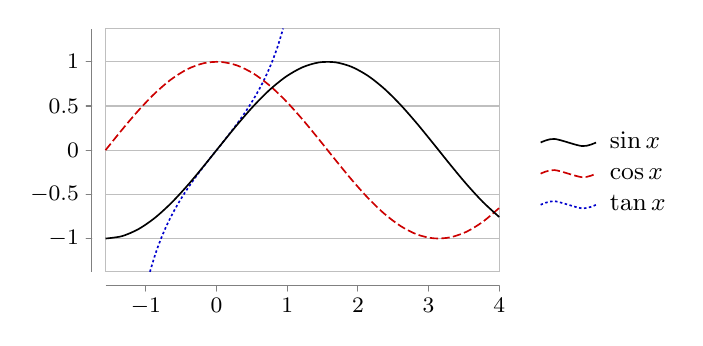
\begin{tikzpicture}
\datavisualization [scientific axes=clean,
                    y axis=grid,
                    visualize as smooth line/.list={sin,cos,tan},
                    style sheet=strong colors,
                    style sheet=vary dashing,
                    sin={label in legend={text=$\sin x$}},
                    cos={label in legend={text=$\cos x$}},
                    tan={label in legend={text=$\tan x$}},
                    data/format=function
                    ]
data [set=sin] {
  var x : interval [-0.5*pi:4];
  func y = sin(\value x r);
}
data [set=cos] {
  var x : interval [-0.5*pi:4];
  func y = cos(\value x r);
}
data [set=tan] {
  var x : interval [-0.3*pi:.3*pi];
  func y = tan(\value x r);
};
\end{tikzpicture}
\end{document}